\chapter{Ex-Vivo Renal MRI}
\label{chap:ex}

\begin{abstract}
	This work was presented as a digital poster at the \ac{ISMRM} 27th Annual Meeting, 2019 \cite{daniel_effects_2019} and as a poster at \ac{UKKW} 2019 \cite{kazmi_determining_2019}. The bespoke analysis pipelines and software developed here were heavily drawn upon in the development of The \ac{UKAT} \cite{nery_ukrin_2020}. This work has also been accepted to be presented at the \ac{ISMRM} 29th Annual Meeting, 2021, \cite{daniel_ukrin_2021}.
\end{abstract}
\acresetall
\newpage
\section{Introduction}

A recurring theme in renal \ac{MRI} studies are the limitations imposed by respiratory motion. Sequences must either be optimised and accelerated to fit within a breath-hold, be hugely slowed down through the use of respiratory triggering or accept the motion artefacts that are inevitable during free-breathing acquisition. Additionally the common trade-off in \ac{MRI} between voxel size, \ac{FOV} and acquisition time becomes all the more limiting within the constraints of respirator motion. While these issues are ever-present in day-to-day clinical practice, they also imped progress, and ultimately, clinical adoption, of techniques in the research phases of their development. Often in research, it is desirable to acquire data of higher quality than would be required in clinical practice. This can be to gain a better understanding of the spacial variance within small structures or acquire best case scenario data with many averages/time points to compare to existing, non-imaging, diagnostic techniques.

In this chapter, techniques for ex-vivo renal \ac{MRI} are developed. These allow research to be conducted without the limitations imposed by respiratory motion and, in future, could be used in the clinic to assess allograft viability prior to transplant.

\subsection{Validation of Multiparametric MRI via a Nephrectomy Model}

Blood and urine tests are commonly used to assess renal health and function however, these are indirect measures and given no indication as the the health of individual kidneys. Consequently, the gold standard in renal diagnostics is a biopsy followed by histological analysis. During a renal biopsy, an area on the patients back is injected with local anaesthetic then, using ultrasound as a guide, a biopsy needle is inserted into the kidney to removing a sample of the tissue. Acquiring the biopsy takes approximately half an hour. The patient is then asked to lie in bed for several hours to minimise the risk of internal bleeding. In approximately 1\% of patients, the bleeding caused will require a blood transfusion and approximately 0.5\% of patients will require embolisation. While these risks are relatively small, the procedure is still an invasive, destructive and time consuming one for the patient thus making it poorly suited for longitudinal monitoring of renal health. Additionally, this method of biopsy is not viable for some patients such as those with coagulopathy or thrombocytopenia due to the increased risk if a hemorrhage occurs or those that are unable to lie prone such as patients who are intubated for respiratory assistance \cite{rathod_safety_2017}. While techniques such as the transjugular renal biopsy have been developed (albeit accidentally after taking a wrong turn at the portal vein while trying to acquire a liver biopsy \cite{mal_transjugular_1990}) to serve these patients, this is a more technically complicated procedure. Finally, the samples acquired via biopsy are very small and thus are often not representative of the entirety of the kidney biopsied, let alone both kidneys.

These drawbacks have provided the incentive for the development of multiparametric renal \ac{MRI} protocols which could prove to be advantageous for both clinicians and patients. A key aspect in the widespread adoption of \ac{MRI} into renal clinical practice, is a full understanding of the interplay between the current histological pipelines and the newly developed \ac{MRI} measurements. While it is possible to correlate biopsy results with \ac{MRI} findings and gain some information as to how different \ac{MRI} measurements vary with tissue properties, this paradigm still suffers from the small tissue sampling volumes outlined above and the inherent difficulties of in-vivo \ac{MRI} data acquisition \cite{leung_could_2017}. An alternative paradigm is to scan the kidney in-vivo to collect typical renal \ac{MRI} data, scan the organ ex-vivo to acquire exquisite \ac{MRI} data of a far higher quality than would be possible in-vivo, then perform whole organ histology on the tissue. These three streams of complimentary data, all acquired from the same organ, eliminate the large issues with currently implemented paradigms, while still being able to reference the data back to clinically feasible measures.


One of the first works correlating multiparametric \ac{MRI} with renal histology was by Inoue \textit{et al}, who found a statistically significant correlation between fibrosis area, as determined from a renal biopsy stained with Masson's trichrome, and \ac{ADC} and \ttwostar in 37 \ac{CKD} patients \cite{inoue_noninvasive_2011}. This was confirmed by Zhao \textit{et al}, who found a strong correlation between \ac{ADC} of both the renal cortex and medulla and histopathological fibrosis score on 25 more \ac{CKD} patients \cite{zhao_assessment_2014}; this study used a more comprehensive histopathology protocol. Feng \textit{et al} also found a correlation between glomerulosclerosis, fibrosis, \ac{FA} and \ac{ADC} in \ac{CKD} subjects \cite{feng_dti_2015}. Friedli \textit{et al} found a significant correlation between cortical-medullary differences in \tone and \ac{ADC} and fibrosis, this was first found in rats, including histology of whole organs rather than just biopsy samples \cite{friedli_new_2016}. The same group then validated this finding in 164 human subjects, correlating with biopsy rather than whole organ \cite{berchtold_validation_2020}.

Outside the renal community, work has been done with registered whole-mount histology and both in-vivo and ex-vivo \ac{MRI}. Jafari \textit{et al} have performed volume matched ex-vivo \ac{QSM} and \ttwostar mapping with whole explant histopathology using the histopathology results to validate predictions of fibrosis using \ac{MRI} \cite{jafari_integrated_2021}. The University of British Columbia group have carried out extensive work correlating histopathology of whole prostatectomy samples with in-vivo \ac{MRI} \cite{sabouri_mr_2017, dhatt_mri_2020}. The same group have also made use of ex-vivo scanning techniques to correlate histopathology with 3T in-vivo data and 7T narrow-bore ex-vivo data \cite{uribe_vivo_2015}. The use of matched histology and \ac{MRI} data is well established in the neuroimaging field \cite{lazari_can_2021} with studies correlating histopathology with diffusion measures \cite{peters_white_2019, moll_multiple_2011, howard_joint_2019, mollink_white_2019}, magnetisation transfer \cite{mottershead_high_2003, seewann_diffusely_2009}, \ac{QSM} \cite{hametner_influence_2018, stuber_myelin_2014} and relaxometry measures \cite{bagnato_untangling_2018, reeves_combined_2016}. Additionally, post processing packages have been developed to enable accurate registration of whole mount histopathology and \ac{MRI} data \cite{huszar_tensor_2019, huszar_automated_2019}.

Thus far, no work has been found comparing whole organ renal histology to in-vivo and ex-vivo \ac{MRI} measurements. The ideal paradigm for this work is to scan patients who are undergoing a nephrectomy as part of their standard clinical care. Briefly, this method would involve scanning a subject pre-operation to acquire a multi-parametric quantitative \ac{MRI} dataset. The subject will then have part of their kidney removed, cancerous tissue will be sent for standard lab tests however, non-cancerous tissue will be immersion fixed in formalin. Equivalent scans assessing the same quantitative parameters as were collected in-vivo will be repeated ex-vivo, however these scans will be at a much higher resolution. Finally, the tissue will be sliced for multi-stain histopathology. This pipeline enables the comparison of tried and tested histological staining that clinicians are used to, albeit with larger sample sizes, with in-vivo quantitative \ac{MRI} data; ex-vivo data acts as an intermediary between histology and in-vivo \ac{MRI} data.

Given the purpose of this paradigm is to compare pre-existing histological analysis with newly developed, but previously documented renal \ac{MRI} protocols, the area that will need the most development is the use of ex-vivo \ac{MRI} to image renal tissue.

\subsection{Assessment of Allograft Viability}

\subsection{Ex-Vivo Protocol Aims}
To enable research into these topics, a range of ex-vivo acquisition techniques with matched in-vivo counterparts was developed with the following aims.

\begin{itemize}
	\item Can be run on widely available hospital hardware
	\item Not take forever
	\item Not need custom coils etc
	\item Not uber time dependent i.e. can scan at any time in a 12 hour window
\end{itemize}

\section{MRI Protocol Development}

As one of the aims in this chapter is for the protocol developed to be able to be performed in a hospital environment, the decision to develop the protocol for use on human scanners rather than pre-clinical scanners was made. Although some hospitals are attached to research institutions with access to pre-clinical \ac{MRI} scanners, this is not the norm. Imaging was performed on a 3T Philips Ingenia system as 3T scanners are available in most European/North American hospitals however some protocols were also developed for a 7T Philips Achieva system to assess the best case scenario ex-vivo images that could be acquired on human scanners, all in-vivo imaging was performed at 3T. All ex-vivo samples were scanned in 32 channel head coils, Figure \ref{fig:ex_head_coil}, as these coils allowed for a whole organ to be imaged while also keeping array elements as close to the signal as possible. In-vivo imaging utilised a 16-channel anterior coil array and 16-channel posterior coil array.

\begin{figure}[H]
	\centering
	\includegraphics[width=0.5\textwidth]{Neph/head_coil.jpg}
	\caption{A sample sat within the 32 channel 3T head coil.}
	\label{fig:ex_head_coil}	
\end{figure}

Sequence development work was performed on formalin fixed porcine samples immersed in \ac{PBS} at room temperature. A more detailed explanation of the sample acquisition and fixation process is provided in Section \ref{sec:ex_tissue_fixation}.

\subsection{Anatomical Scans}

To make use of the layer based analysis techniques outlined in Section \ref{sec:ex_layers} and calculate \ac{TKV} a high resolution, whole kidney coverage anatomical scan is required to segment the kidney from surrounding tissue/\ac{PBS}. In-vivo, the \ttwo weighted structural scan from Chapter \ref{chap:ML} is used. The ex-vivo protocol is outlined in Table \ref{tab:ex_anatomical}; this scan was also used to plan subsequent ex-vivo scans.

\begin{table}[H]
	\centering
	\begin{tabularx}{1.0\textwidth}{|X|X|X|}
		\hline
		Parameter                          & 3T Ex-Vivo     & 3T In-Vivo      \\ \hline
		Voxel Size                         & 1 x 1 x 1      & 1.5 x 1.5 x 5   \\ \hline
		FoV                                & 192 x 192 x 60 & 350 x 350 x 71  \\ \hline
		Acquisition Mode                   & 3D             & M2D             \\ \hline
		TE                                 & 3.7            & 60              \\ \hline
		TR                                 & 8.1            & 1300            \\ \hline
		Flip Angle                         & 15             & 90              \\ \hline
		Bandwidth                          & 191.5          & 792.3           \\ \hline
		NSA                                & 1              & 1               \\ \hline
		Fold-over Suppression Oversampling & N/A            & 150             \\ \hline
		Sense                              & 2 RL, 2AP      & 2.5             \\ \hline
		Halfscan                           & 0.625          & N/A             \\ \hline
		Fast Imaging Mode                  & TFE            & TSE             \\ \hline
		TFE Factor                         & 143            & N/A             \\ \hline
		Shot Interval                      & 4000           & N/A             \\ \hline
		Acquisition Time                   & 53 sec         & 17 sec (1 x BH) \\ \hline
	\end{tabularx}
	\caption{Acquisition parameters for anatomical scans.}
	\label{tab:ex_anatomical}
\end{table}

\subsection{\tone Mapping}
% Acquisition
\tone mapping protocols were developed for both 3T and 7T systems using an ultrafast gradient echo inversion recovery scheme. The basics of this sequence and \tone mapping are outlined in Section \ref{subsec:theory_t1}. An example of the acquisitions at each inversion time is shown in Figure \ref{fig:ex_ir_data}. The sequence parameters at both 3T and 7T are shown in Table \ref{tab:ex_t1_mapping}.
\begin{figure}[H]
	\centering
	\includegraphics[width=1\textwidth]{Neph/Individual_TI.eps}
	\caption{Acquisitions at each of the \ac{TI} at 7T.}
	\label{fig:ex_ir_data}	
\end{figure}

\begin{table}[H]
	\centering
	\begin{tabularx}{1.0\textwidth}{|X|X|X|X|}
		\hline
		Parameter                            & 3T Ex-Vivo                                         & 7T Ex-Vivo                                         & 3T In-Vivo                                                         \\ \hline
		Voxel Size                           & 0.7 x 0.7 x 1.0                                    & 0.6 x 0.6 x 0.6                                    & 3 x 3 x 5                                                          \\ \hline
		FoV                                  & 160 x 160 x 50                                     & 192 x 170 x 24                                     & 288 x 288 x 25                                                     \\ \hline
		Acquisition Mode                     & 3D                                                 & 3D                                                 & MS                                                                 \\ \hline
		TE                                   & 5.1                                                &                                                    & 27                                                                 \\ \hline
		TR                                   & 11                                                 &                                                    & 5000                                                               \\ \hline
		TI                                   & 400, 500, 750, 900,   1100, 1300, 1500, 2000, 2600 & 250, 500, 750, 900,   1100, 1300, 1500, 2000, 3000 & 0, 100, 200, 300,   400, 500, 600, 700, 800, 900, 1000, 1100, 1300 \\ \hline
		Flip Angle                           & 8                                                  & 8                                                  & 90                                                                 \\ \hline
		Bandwidth                            & 134.4                                              &                                                    & 39.3                                                               \\ \hline
		NSA                                  & 1                                                  & 2                                                  & 1                                                                  \\ \hline
		Fold-over Suppression   Oversampling & 75                                                 & N/A                                                & N/A                                                                \\ \hline
		Sense                                & 2.5 RL, 1 AP                                       & 2 RL,1.5 AP                                        & 2.3                                                                \\ \hline
		Halfscan                             & N/A                                                & N/A                                                & 0.851                                                              \\ \hline
		Fast Imaging Mode                    & TFE                                                & TFE                                                & EPI                                                                \\ \hline
		TFE Factor                           & 64                                                 & 240                                                & N/A                                                                \\ \hline
		Shot Interval                        & 3000                                               & 8000                                               & N/A                                                                \\ \hline
		Acquisition Time                     & 1 hr 20 min 20 sec                                 &                                                    & 1 min 10 sec (Trig)                                                \\ \hline
	\end{tabularx}
	\caption{\tone mapping protocols and 3T and 7T.}
	\label{tab:ex_t1_mapping}
\end{table}

After a 180$\degree$ inversion, t`he signal sampled at each inversion time is proportional to the modulus of the true longitudinal magnetisation, as such, the true dynamic range of the inversion recovery is not sampled. This factor means there is ambiguity as to the polarity of signals near the null point (zero crossing) and can lead to a decreased accuracy when fitting for \tone as any algorithm is essentially having to fit an extra parameter in the form of the null point. 

If the phase of the signal has been saved, the polarity of the magnitude can be corrected using the methods of Szumowski \textit{et al} \cite{szumowski_signal_2012} thus increasing accuracy by increasing dynamic range and removing ambiguity as to the location of the null point for each voxel. Phase data is only accurate if partial Fourier acquisition acceleration techniques (Section \ref{subsec:theory_partial_fourier}), known as halfscan, are not utilised however, because these acceleration methods result in a decreased \ac{SNR} they would not be used ex-vivo anyway.

\begin{figure}[H]
	\centering
	\includegraphics[width=0.5\textwidth]{neph/magnitude_correct.pdf}
	\caption{The raw signal recorded from a single voxel and the magnitude corrected signal with increased dynamic range.}
	\label{fig:ex_sig_mag_correction}	
\end{figure}

Once the data has been polarity corrected, a voxel by voxel, least squares trust region reflective method is used to fit the data from each voxel to Equation \eqref{eq:ex_t1} to estimate the \tone and $M_0$ of the tissue and an uncertainty in the fit \cite{branch_subspace_1999}.

\begin{equation}
	S(TI) = M_0\left(1-2 \cdot e^{-\sfrac{TI}{\tone}}\right)
	\label{eq:ex_t1}
\end{equation}

Using these techniques, the \tone of ex-vivo samples could be calculated at both 3T and 7T, Figure \ref{fig:ex_t1_maps}. For in-vivo acquisitions, halfscan was used and as such magnitude correction could not be employed. As such, in-vivo data was fit to the modulus of Equation \eqref{eq:ex_t1}.
 
\begin{figure}[H]
	\centering
	\begin{subfigure}[c]{0.47\textwidth}
		\centering
		\includegraphics[width=1\textwidth]{Neph/T1_map_3T.eps}
		\caption{}
		\label{fig:ex_t1_map_3t}
	\end{subfigure}
	\hfill
	\begin{subfigure}[c]{0.47\textwidth}
		\centering
		\includegraphics[width=1\textwidth]{Neph/T1_map_7T.eps}
		\caption{}
		\label{fig:ex_t1_map_7t}
	\end{subfigure}
	\caption{Example \tone maps generated at both 3T (\subref{fig:ex_t1_map_3t}) and 7T (\subref{fig:ex_t1_map_7t}).}
	\label{fig:ex_t1_maps}
\end{figure}

\subsection{\ttwo Mapping}

\ttwo mapping makes use of the \ac{GraSE} sequence developed in Chapter \ref{chap:t2_mapping}. This sequence was only implemented at 3T, an example of the acquisitions at each \ac{TE} is shown in Figure \ref{fig:ex_t2_raw_data} and the sequence parameters are shown in Table \ref{tab:ex_t2_mapping}. The very wide range of \ac{TE} sampled ex-vivo will enable future multi-exponential analysis of the data allowing for a more accurate quantification of the long \ttwo components of the tissue \cite{bjarnason_analyzennls_2010, sabouri_mr_2017}.

\begin{figure}[H]
	\centering
	\includegraphics[width=0.8\textwidth]{Neph/T2_Individual_TE.eps}
	\caption{Acquisitions of an ex-vivo sample at each of the \ac{TE}.}
	\label{fig:ex_t2_raw_data}	
\end{figure}

\begin{table}[H]
	\centering
	\begin{tabularx}{1.0\textwidth}{|X|X|X|}
		\hline
		Parameter                          & 3T Ex-Vivo      & 3T In-Vivo         \\ \hline
		Voxel Size                         & 0.7 x 0.7 x 1.0 & 3 x 3 x 5          \\ \hline
		FoV                                & 160 x 160 x 20  & 288 x 288 x 25     \\ \hline
		Acquisition Mode                   & MS              & MS                 \\ \hline
		TE                                 & 31:15.8:489.9   & 11:5.6:179         \\ \hline
		TR                                 & 3000            & 3000               \\ \hline
		Flip Angle                         & 90              & 90                 \\ \hline
		Bandwidth                          & 118.9           & 427.9              \\ \hline
		NSA                                & 2               & 1                  \\ \hline
		Fold-over Suppression Oversampling & 75              & 66                 \\ \hline
		Sense                              & 2.55            & 2.55               \\ \hline
		Halfscan                           & N/A             & N/A                \\ \hline
		Fast Imaging Mode                  & GraSE           & GraSE              \\ \hline
		TFE Factor                         & 30              & 30                 \\ \hline
		EPI Factor                         & 3               & 3                  \\ \hline
		Startup Echoes                     & 1               & 1                  \\ \hline
		Acquisition Time                   & 30 min 30 sec   & 3 min 9 sec (Trig) \\ \hline
	\end{tabularx}
	\caption{\ttwo mapping sequence parameters.}
	\label{tab:ex_t2_mapping}
\end{table}

\ttwo maps are generated on a voxel by voxel basis using a least squares trust region reflective methods to fit the data to Equation \eqref{eq:ex_t2} to estimate \ttwo and $M_0$. 
\begin{equation}
	S(TE) = M_0 \cdot e^{-\sfrac{TE}{\ttwo}}
	\label{eq:ex_t2}
\end{equation}
As outlined in Section \ref{subsec:t2_fitting_methods_results} multiple methods of estimating \ttwo were compared with the basic two parameter fit delivering the most desirable results. Using this pipeline, \ttwo maps could be generated, an example of which is shown in Figure \ref{fig:ex_t2_map}. While partial voluming has been minimised by keeping voxel sizes small, the use of multi-exponential fitting models should be explored in future. This would allow the long \ttwo components of the signal, such as the signal from \ac{PBS} to be modelled separately to the renal tissue, thus increasing accuracy.

\begin{figure}[H]
	\centering
	\includegraphics[width=0.7\textwidth]{Neph/ex_vivo_t2_map.pdf}
	\caption{An example ex-vivo \ttwo map acquired using the scheme above. This sample had been formalin fixed and stored in \ac{PBS} for multiple months, hence the lack of contrast between cortical and medullary tissue.}
	\label{fig:ex_t2_map}
\end{figure}

\subsection{\ttwostar Mapping}

\ttwostar acquisition is performed using a simple multi-slice gradient echo sequence as outlined in Section \ref{subsubsec:theory_ge} and was developed at both 3T and 7T. The acquisition parameters are shown in Table \ref{tab:ex_t2star_mapping}. In addition to the magnitude data saved for \ttwostar mapping, the phase data is also saved to allow a \ac{QSM} pipeline to be developed in future.

\begin{figure}[H]
	\centering
	\includegraphics[width=0.8\textwidth]{Neph/Individual_TE.eps}
	\caption{Acquisitions at each of the \ac{TE} at 7T.}
	\label{fig:ex_t2star_raw_data}	
\end{figure}

\begin{table}[H]
	\centering
	\begin{tabularx}{1.0\textwidth}{|X|X|X|X|}
		\hline
		Parameter                          & 3T Ex-Vivo      & 7T Ex-Vivo                     & 3T In-Vivo      \\ \hline
		Voxel Size                         & 0.7 x 0.7 x 1.0 & 0.5 x 0.5 x 1                  & 1.5 x 1.5 x 5   \\ \hline
		FoV                                & 160 x 160 x 25  & 145 x 145 x 10                 & 288 x 288 x 25  \\ \hline
		Acquisition Mode                   & MS              & MS                             & MS              \\ \hline
		TE                                 & 15:5:50         & 10, 13, 16, 19, 22, 25, 28, 30 & 5:3:38          \\ \hline
		TR                                 & 697             &                                & 79              \\ \hline
		Flip Angle                         & 38              & 38                             & 25              \\ \hline
		Bandwidth                          & 35 - 56         &                                & 1328.6          \\ \hline
		NSA                                & 1               & 3                              & 1               \\ \hline
		Fold-over Suppression Oversampling & 75              & N/A                            & 144             \\ \hline
		Sense                              & 2               & 2                              & 2               \\ \hline
		Halfscan                           & N/A             & N/A                            & N/A             \\ \hline
		Fast Imaging Mode                  & None            & None                           & None            \\ \hline
		Acquisition Time                   & 46 min 25 sec   &                                & 47 sec (3 x BH) \\ \hline
	\end{tabularx}
	\caption{Acquisition parameters for \ttwostar mapping sequences at 3T and 7T.}
	\label{tab:ex_t2star_mapping}
\end{table}

Estimation of \ttwostar can be performed via two different methods, fitting to a two parameter exponential (Equation \eqref{eq:ex_t2star}) or performing a weighted linear fit to the natural logarithm of the signal. The latter of these methods is far less computationally intensive and as such, runs much quicker.

\begin{equation}
	S(TE) = M_0 \cdot e^{-\sfrac{TE}{\ttwostar}}
	\label{eq:ex_t2star}
\end{equation}

The acquisition parameters of the 3T ex-vivo protocol were simulated to compare the two fitting methods using Monte Carlo techniques. The linear fit produces a slightly greater \ac{CoV} than the exponential fit at lower \ttwostar, Figure \ref{fig:ex_t2star_sim_cov}. Additionally, the relative error, defined by Equation \eqref{eq:ex_re}, has a greater magnitude below 20 ms when fitting with the linear fit than the exponential fit, Figure \ref{fig:ex_t2star_sim_mre}. The \ttwostar we expect from the kidneys at 3T is greater than 20 ms so in the interests of computational efficiency, the linear fitting method was used.

\begin{equation}
	\textup{Relative Error} = \frac{t_{2\; \textup{fit}}^{*} - t_{2\; \textup{simulated}}^{*}}{t_{2\; \textup{simulated}}^{*}}
	\label{eq:ex_re}
\end{equation}

\begin{figure}[H]
	\centering
	\begin{subfigure}[c]{0.47\textwidth}
		\centering
		\includegraphics[width=1\textwidth]{Neph/t2star_sim_cov.pdf}
		\caption{}
		\label{fig:ex_t2star_sim_cov}
	\end{subfigure}
	\hfill
	\begin{subfigure}[c]{0.47\textwidth}
		\centering
		\includegraphics[width=1\textwidth]{Neph/t2star_sim_mre.pdf}
		\caption{}
		\label{fig:ex_t2star_sim_mre}
	\end{subfigure}
	\caption{Simulations to ascertain the accuracy of each \ttwostar fitting algorithm over a range of \ttwostar.}
	\label{fig:ex_t2star_sim}
\end{figure}

Using the acquisition and post processing steps above, \ttwostar maps can be generated, examples of which are shown in Figure \ref{fig:ex_t2star_maps}.

\begin{figure}[H]
	\centering
	\begin{subfigure}[c]{0.47\textwidth}
		\centering
		\includegraphics[width=1\textwidth]{Neph/T2star_map_3T.eps}
		\caption{}
		\label{fig:ex_t2star_map_3t}
	\end{subfigure}
	\hfill
	\begin{subfigure}[c]{0.47\textwidth}
		\centering
		\includegraphics[width=1\textwidth]{Neph/T2star_map_7T.eps}
		\caption{}
		\label{fig:ex_t2star_map_7t}
	\end{subfigure}
	\caption{An example \ttwostar map acquired at 3T (\subref{fig:ex_t2star_map_3t}) and 7T (\subref{fig:ex_t2star_map_7t}) fit using the weighted fit to the natural logarithm of the signal.}
	\label{fig:ex_t2star_maps}
\end{figure}

\subsection{\acl*{ADC} Mapping}
\label{subsec:ex_adc}

The underlying principles of diffusion imaging are outlined in Section \ref{subsec:theory_diffusion}, here \ac{DWI} is performed using a single shot \ac{SE}-\ac{EPI} sequence over a range of b-values applied in three orthogonal directions. By acquiring diffusion gradients in three different directions and calculating the mean, the effects of diffusion anisotropy can be minimised. The sequence was developed for 3T systems with a schematic of the sequence shown in Figure \ref{fig:ex_adc_psd} and the sequence parameters summarised in Table \ref{tab:ex_adc_mapping}. 

\begin{figure}[H]
	\centering
	\includegraphics[width=0.8\textwidth]{Theory/Diffusion/diffusion_psd_epi.pdf}
	\caption{A schematic of the \ac{SE}-\ac{EPI} sequence used for \ac{ADC} mapping. This block is repeated multiple times with diffusion gradients applied in different directions and with different strengths.}
	\label{fig:ex_adc_psd}	
\end{figure}

\begin{table}[H]
	\centering
	\begin{tabularx}{1.0\textwidth}{|X|X|X|}
		\hline
		Parameter                          & 3T Ex-Vivo                                                                       & 3T In-Vivo                                                                       \\ \hline
		Voxel Size                         & 1.5 x 1.5 x 1.5                                                                  & 1.5 x 1.5 x 5                                                                    \\ \hline
		FoV                                & 160 x 160 x 51                                                                   & 288 x 288 x 25                                                                   \\ \hline
		Acquisition Mode                   & MS                                                                               & MS                                                                               \\ \hline
		TE                                 & 72                                                                               & 71                                                                               \\ \hline
		TR                                 & 1800                                                                             & 1800                                                                             \\ \hline
		b-values                           & 0, 5, 15, 30, 45, 60, 75, 90, 105, 120, 135, 150, 175,   200, 300, 400, 500, 600 & 0, 5, 15, 30, 45, 60, 75, 90, 105, 120, 135, 150, 175,   200, 300, 400, 500, 600 \\ \hline
		Flip Angle                         & 90                                                                               & 90                                                                               \\ \hline
		Bandwidth                          & 13.2                                                                             & 13.7                                                                             \\ \hline
		NSA                                & 1                                                                                & 1                                                                                \\ \hline
		Fold-over Suppression Oversampling & 75                                                                               & N/A                                                                              \\ \hline
		Sense                              & 2.3                                                                              & 2.3                                                                              \\ \hline
		Halfscan                           & 0.676                                                                            & 0.676                                                                            \\ \hline
		Fast Imaging Mode                  & EPI                                                                              & EPI                                                                              \\ \hline
		EPI Factor                         & 91                                                                               & 83                                                                               \\ \hline
		Phase Encode Direction             & L then R                                                                         & L then R                                                                         \\ \hline
		Acquisition Time                   & 9 min 44 sec                                                                     & 2 min 42 sec (Trig)                                                              \\ \hline
	\end{tabularx}
	\caption{\ac{ADC} mapping acquisition parameters.}
	\label{tab:ex_adc_mapping}
\end{table}

The diffusion sensitising block of the pulse sequence is time consuming and as such necessitates the use of fast image techniques, \ac{EPI} is the simplest to implement however is not without drawbacks. It suffers from geometric distortions, particularly in the phase encode direction, due to inhomogeneities in the $B_0$ field cause by susceptibility differences. These geometric distortions can be problematic for this paradigm as the ability to correlate, on a voxel by voxel basis, parameters acquired with different sequences is at the core of multiparametric \ac{MRI}. Geometric distortions make this impossible. The susceptibility of \ac{PBS} and renal tissue is similar however there is a very large difference between the \ac{PBS} and surrounding air and as such, distortions can be problematic. 

As the distortions are predominantly in the phase encode direction, by inverting the direction of the phase encode blips, the direction of the distortion can be reversed, Figure \ref{fig:ex_epi_distortion_overlay}. By acquiring images with both phase encode directions the underlying field map can be estimated and used to undistort the data \cite{andersson_how_2003}. This process can be carried out using \ac{FSL} ``topup'' however, as this tool was designed for work in the brain, a custom configuration to perform more iterations of the field estimation algorithm with a greater degree of regularisation is required. 

Although in some cases it is possible ot acquire only the b0 image in both phase encode directions, calculate the displacement field, then apply this field to other b-values, it was decided that the $\sqrt{2}$ \ac{SNR} increase of acquiring two volumes and averaging them is beneficial. Additionally if, in the case of in-vivo data, there are issues with motion in the b0 volumes, then another diffusion weighting can be used to estimate the displacement, thus adding inherent redundancy to the pipeline.

\begin{figure}[H]
	\centering
	\begin{subfigure}[c]{0.47\textwidth}
		\centering
		\includegraphics[width=1\textwidth]{Neph/epi_distortion_overlay.png}
		\caption{}
		\label{fig:ex_epi_distortion_overlay}
	\end{subfigure}
	\hfill
	\begin{subfigure}[c]{0.47\textwidth}
		\centering
		\includegraphics[width=1\textwidth]{Neph/epi_distortion_corrected.png}
		\caption{}
		\label{fig:ex_epi_distortion_corrected}
	\end{subfigure}
	\caption{(\subref{fig:ex_epi_distortion_overlay}) b0 images collected with opposing phase encode directions overlay in red and blue. (\subref{fig:ex_epi_distortion_corrected}) A composite image with \ac{EPI} distortions corrected using topup.}
	\label{fig:ex_epi_distortion}
\end{figure}

\begin{figure}[H]
	\centering
%	\includegraphics[width=0.8\textwidth]{}
	\missingfigure{Individual b-values}
	\caption{Distortion corrected images at each b-value.}
	\label{fig:ex_adc_raw_data}	
\end{figure}
%\subsubsection{Optimising b-values}
%
%As with many quantitative \ac{MRI} techniques, there is a balance with \ac{ADC} mapping between acquisition time and quantitative accuracy. By sampling more b-values, the estimation of \ac{ADC} becomes more accurate however this inherently takes longer. To ascertain the optimum number of b-values to collect and their locations a methodical search was conducted.
%
%\ac{ADC} data was collected from two different subjects using 16 b-values, more than would normally be collected, with \ac{ADC} maps being generated using all 16 values. \ac{ADC} maps were then fit for every combination and number of b-values using more than six of the available values. The resulting \ac{ADC} maps were then compared to the map generated using the full dataset.

The average of the three directions at each b-value and phase encode direction is calculated. \ac{EPI} distortion correction is performed on both ex-vivo and in-vivo data using topup to enable accurate voxel by voxel comparison of \ac{ADC} to other quantitative parameters. The natural logarithm of the distortion corrected signal from each voxel over each b-value is taken and a linear least squares fit performed. This enables a quick estimation of \ac{ADC} and an uncertainty in the fit. 

Using these techniques, the \ac{ADC} of both in-vivo and ex-vivo renal tissue can be calculated, Figure \ref{fig:ex_adc_maps} with no geometric distortions. Although not implemented here, the large number of low b-values sampled should make estimations of more advance diffusion parameters possible such as fitting the data to an \ac{IVIM} model \cite{le_bihan_separation_1988}.

\begin{figure}[H]
	\centering
	\begin{subfigure}[c]{0.47\textwidth}
		\centering
		\includegraphics[width=1\textwidth]{Neph/in_vivo_adc.pdf}% 20190926
%		\missingfigure{In-Vivo ADC Map}
		\caption{}
		\label{fig:ex_adc_maps_in_vivo}
	\end{subfigure}
	\hfill
	\begin{subfigure}[c]{0.47\textwidth}
		\centering
		\includegraphics[width=1\textwidth]{Neph/ex_vivo_adc.pdf}% 20190923
%		\missingfigure{Ex-Vivo ADC Map 20190923}
		\caption{}
		\label{fig:ex_adc_maps_ex_vivo}
	\end{subfigure}
	\caption{\ac{ADC} maps acquired of both an in-vivo subject (\subref{fig:ex_adc_maps_in_vivo}) and ex-vivo sample (\subref{fig:ex_adc_maps_ex_vivo}).}
	\label{fig:ex_adc_maps}
\end{figure}




\subsection{\acl*{DTI}}

\ac{ADC} maps provide an understanding as to how readily molecules can diffuse through a tissue, however they do not provide any information as to what directions the molecules are travelling, to measure this, \ac{DTI} is used. The renal group at \ac{SPMIC} had no existing high resolution in-vivo (or ex-vivo) \ac{DTI} protocol, as such this was specifically developed for this paradigm.

The acquisition scheme used is very similar to that in Section \ref{subsec:ex_adc}, a single shot \ac{SE}-\ac{EPI} scheme with monopolar diffusion gradients. The difference lies in the fact that, rather than acquiring a large range of b-values over three different directions, only a b0 and one other b-value are acquired over a minimum of six directions although in practice, many more. This is known as a single shell \ac{DTI} scheme. As the diffusivity in, for example, the positive $x$ direction is the same as the negative $x$ direction most \ac{DTI} schemes acquire a hemisphere of directions, however, to apply additional image deformation correction techniques outlined below, diffusion vectors were acquired over a full sphere, Figure \ref{fig:ex_dti_vectors}.

\begin{figure}[H]
	\centering
	\begin{subfigure}[c]{0.47\textwidth}
		\centering
		\includegraphics[width=1\textwidth]{Neph/64_dir_hemispherical.pdf}
		\caption{}
		\label{fig:ex_dti_vectors_half}
	\end{subfigure}
	\hfill
	\begin{subfigure}[c]{0.47\textwidth}
		\centering
		\includegraphics[width=1\textwidth]{Neph/64_dir_spherical.pdf}
		\caption{}
		\label{fig:ex_dti_vectors_full}
	\end{subfigure}
	\caption{(\subref{fig:ex_dti_vectors_half}) 64 diffusion directions acquired over a hemisphere (\subref{fig:ex_dti_vectors_full}) 64 diffusion directions acquired over a full sphere as used in this chapter. b0 is shown in orange with subsequent b-values shown in blue. }
	\label{fig:ex_dti_vectors}
\end{figure}

Mathematically, \ac{DTI} is estimating the tensor, $\mathscr{D}$ in equation \eqref{eq:ex_diffusion_tensor} where $D_{xx}$, $D_{yy}$ and $D_{zz}$ represent diffusivity along the $x$, $y$ and $z$ directions in the lab frame and are equivalent to the three directions sampled in Section \ref{subsec:ex_adc}. $D_{yx}$, $D_{zx}$ and $D_{zy}$ represent diffusivity between the principle axis of the lab frame, as $\mathscr{D}$ is symmetric, $D_{yx} \equiv D_{xy}$, $D_{zx} \equiv D_{xz}$ etc, hence \ac{DTI} can be performed by only sampling a hemisphere of diffusion vectors.

\begin{equation}
	\mathscr{D} = 
	\begin{bmatrix}
		D_{xx} & D_{xy} & D_{xz}\\ 
		D_{yx} & D_{yy} & D_{yz}\\ 
		D_{zx} & D_{zy} & D_{zz}
	\end{bmatrix}
\label{eq:ex_diffusion_tensor}
\end{equation}

Like the \ac{ADC} sequence, a full dataset is acquired with both opposing phase encode directions to assist with geometric distortion correction. A summary of the sequence parameters is shown in Table \ref{tab:ex_dti_mapping}. 

\begin{table}[H]
	\centering
	\begin{tabularx}{1.0\textwidth}{|X|X|X|}
		\hline
		Parameter                          & 3T Ex-Vivo      & 3T In-Vivo          \\ \hline
		Voxel Size                         & 2.3 x 2.3 x 2.3 & 3 x 3 x 3           \\ \hline
		FoV                                & 160 x 160 x 51  & 288 x 288 x 60      \\ \hline
		Acquisition Mode                   & MS              & MS                  \\ \hline
		TE                                 & 85              & 82                  \\ \hline
		TR                                 & 5100            & 5100                \\ \hline
		b-values                           & 0, 600          & 0, 600              \\ \hline
		Directions                         & 128             & 64                  \\ \hline
		Flip Angle                         & 90              & 90                  \\ \hline
		Bandwidth                          & 17.1            & 30.5                \\ \hline
		NSA                                & 2               & 1                   \\ \hline
		Fold-over Suppression Oversampling & 100             & N/A                 \\ \hline
		Sense                              & 2               & 2                   \\ \hline
		Halfscan                           & 0.609           & 0.609               \\ \hline
		Fast Imaging Mode                  & EPI             & EPI                 \\ \hline
		EPI Factor                         & 79              & 47                  \\ \hline
		Phase Encode Direction             & L then R        & L then R            \\ \hline
		Acquisition Time                   & 52 min 42 sec   & 8 min 10 sec (Trig) \\ \hline
	\end{tabularx}
	\caption{\ac{DTI} acquisition parameters.}
	\label{tab:ex_dti_mapping}
\end{table}

The large number of diffusion directions sampled makes additional geometric distortion possible. The rapidly switching fields of the diffusion sequence induce eddy currents in the sample, which in turn induce an opposing magnetic field. This leads to off-resonance distortions in the image. To combat this \ac{FSL}s ``eddy'' can be used \cite{andersson_integrated_2016}. This tool was developed with the brain data from the Human Connectome Project in mind however \cite{andersson_non-parametric_2015}, here is is successfully used to reduce geometric distortions in ex-vivo and in-vivo \ac{DTI} data and subject motion in the in-vivo data. The tools performance is optimal when b-vectors are distributed over a full sphere as this results is approximately opposing eddy current distortions and as such, makes estimation of the deformation more accurate.

Once the raw data has been processed with topup and eddy, quantitative maps can be generated. Eigenvalues ($\lambda_1$, $\lambda_2$, $\lambda_3$) and eigenvectors ($\epsilon_1$, $\epsilon_2$, $\epsilon_3$) are calculated for each diffusion tensor, $\mathscr{D}$. \ac{FA} maps can be calculated from equation \eqref{eq:ex_fa}. Here it can be seen that if $\lambda_1 = \lambda_2 = \lambda_3$, as is the case for isotropic diffusion, \ac{FA} tends to 0. An example renal \ac{FA} map is shown in Figure \ref{fig:ex_dti_fa} where bright areas represent areas of higher \ac{FA} and therefore more anisotropic diffusion.

\begin{equation}
	\textup{FA} = \sqrt{\frac{\left(\lambda_1 - \lambda_2\right)^2 + \left(\lambda_2 - \lambda_3\right)^2 + \left(\lambda_1 - \lambda_3\right)^2}{2\left( \lambda_1^2 + \lambda_2^2 + \lambda_3^2\right)}}
		\label{eq:ex_fa}
\end{equation}

\ac{FA} can also be used to create fibre direction maps as shown in Figure \ref{fig:ex_dti_fa_rgb}. Here the colour is determined by the direction of the principal eigenvector, $\epsilon_1$, the primary direction of diffusion, and the brightness is modulated by \ac{FA}. As the name suggests, these maps provide a visual indication as to the direction diffusion is occurring in a tissue and how strongly it is constrained to that single direction.

The final voxel based map produced using the \ac{DTI} data is an \ac{ADC} map, often called \ac{MD} in \ac{DTI} literature. This is calculated using equation \eqref{eq:ex_dti_md} and an example is shown in Figure \ref{fig:ex_dti_md}. All three of these voxel based maps are generated using \ac{FSL}.

\begin{equation}
	\textup{MD} = \frac{\left( \lambda_1 + \lambda_2 + \lambda_3 \right)}{3}
	\label{eq:ex_dti_md}
\end{equation}

\begin{figure}[H]
	\centering
	\begin{subfigure}[c]{0.31\textwidth}
		\centering
			\includegraphics[width=1\textwidth]{Neph/in_vivo_fa.png}
		\caption{}
		\label{fig:ex_dti_fa}
	\end{subfigure}
	\hfill
	\begin{subfigure}[c]{0.31\textwidth}
		\centering
			\includegraphics[width=1\textwidth]{Neph/in_vivo_fa_rgb.png}
		\caption{}
		\label{fig:ex_dti_fa_rgb}
	\end{subfigure}
	\hfill	
	\begin{subfigure}[c]{0.31\textwidth}
		\centering
			\includegraphics[width=1\textwidth]{Neph/in_vivo_md.png}
		\caption{}
		\label{fig:ex_dti_md}
	\end{subfigure}
	\caption{\ac{FA} (\subref{fig:ex_dti_fa}), fibre direction (\subref{fig:ex_dti_fa_rgb}) and \ac{MD} (\subref{fig:ex_dti_md}) maps generated from the same in-vivo \ac{DTI} data.}
	\label{fig:ex_dti_maps}
\end{figure}

An extension of the fibre direction map is tractography, a technique that can remove the simplification that a voxel has a single direction of diffusion. Even at the highest resolutions achievable with \ac{MRI}, the biological structures dictating diffusion are orders of magnitude smaller than the resolving power of \ac{MRI} and as such multiple mechanisms can occur in a single voxel e.g. crossing of neurons or microvascular. In the brain this technique is used to visualise nerve tracts and connectivity within the brain; in the kidneys it can be used to visualise the coherent motion of renal processes. Tractography calculations are performed using the open-source python package Dipy \cite{garyfallidis_dipy_2014} and the resulting tracts were visualised using TrackVis \cite{wang_diffusion_2007}.

To model multiple fibres entering and exiting a voxel, a more sophisticated model than simply looking at the principle eigenvector is required. This takes the form of an \ac{ODF} which can be thought of as the probability a fibre will enter or exit a voxel through a specific solid angle. \acp{ODF} can be visualised as isosurfaces where the surface represent all points of equal probability, example \acp{ODF} are shown in Figure \ref{fig:ex_dti_odf}. Techniques such as Q-ball imaging \cite{descoteaux_regularized_2007, hess_q-ball_2006} and diffusion spectrum imaging \cite{descoteaux_regularized_2007} can be used to estimate the \ac{ODF} however these methods tend to require high b-values and as such a lower \ac{SNR} acquisition making them less suitable to abdominal imaging. Instead a constrained spherical deconvolution method is used \cite{tournier_direct_2004, tournier_robust_2007, tax_recursive_2014}.

\begin{figure}[H]
	\centering
	\begin{subfigure}[c]{0.47\textwidth}
		\centering
		\includegraphics[width=1\textwidth]{Neph/csd_odfs.png}
		\caption{}
		\label{fig:ex_dti_odfs}
	\end{subfigure}
	\hfill
	\begin{subfigure}[c]{0.47\textwidth}
		\centering
		\includegraphics[width=1\textwidth]{Neph/csd_odf_b0.png}
		\caption{}
		\label{fig:ex_dti_odf_b0}
	\end{subfigure}
	\caption{The \acp{ODF} for a small number of voxels of renal tissue (\subref{fig:ex_dti_odfs}) and the corresponding b0 image to help visualise the part of the kidney the data is coming from (\subref{fig:ex_dti_odf_b0}).}
	\label{fig:ex_dti_odf}
\end{figure}

The peak values of \acp{ODF} are calculated and used to generate streamlines which represent the tracts of coherent diffusion. The calculation of streamline paths is performed using the \ac{EuDX} method \cite{garyfallidis_towards_2013}. This tractography pipeline and its many hyper-parameters are best summarised in code form and as such are included in Appendix \ref{app:tractography_pipeline}. The results of this processing pipeline are tractograms as shown in Figure \ref{fig:ex_dti_tracts}.

\begin{figure}[H]
	\centering
	\includegraphics[width=.9\textwidth]{Other/DTI/img5c.png}
	\caption{Example tractography generated using the above protocol.}
	\label{fig:ex_dti_tracts}
\end{figure}

As this tractography protocol was developed from scratch, both acquisition and the post processing pipeline were verified in the brain. Tractography is a far more mature technique in neuroimaging and as such, verification that the pipeline produces reasonable results on a more familiar anatomy lends confidence to the tractograms produced of the kidneys. The \ac{FOV} of the acquisition was adjusted to cover the whole brain but all other parameters were kept constant. The resulting maps and tractogram were all as expected, an example tractogram of the brain produced using this pipeline is shown in Figure \ref{fig:ex_dti_brain_tracts}.

\begin{figure}[H]
	\centering
	\includegraphics[width=0.8\textwidth]{Neph/brain_tracts.png}
	\caption{A tractogram of the brain produced to verify the \ac{DTI} acquisition and post-processing scheme developed for the kidneys produces expected results within a structure more commonly the subject of tractography.}
	\label{fig:ex_dti_brain_tracts}	
\end{figure}

Renal in-vivo results were compared to those in literature and found to be in agreement \cite{gurses_diffusion_2011, jaimes_diffusion_2014, notohamiprodjo_diffusion_2010}. Additionally, renal features with a known structure can be observed in the tractograms such as the radial structure of the medullary pyramids, Figure \ref{fig:ex_dti_medulla_tracts}.

\begin{figure}[H]
	\centering
	\includegraphics[width=0.7\textwidth]{Neph/medullary_tracts_2.png} % 20190926
	\caption{The medullary pyramids observed in tractography.}
	\label{fig:ex_dti_medulla_tracts}	
\end{figure}

An area that still needs further development is the ex-vivo \ac{DTI} protocol. There are promising early results however ex-vivo diffusion imaging poses additional difficulties. During the fixation process, methyl bridges cross link with proteins within the tissue stiffening it and causing a small amount of shrinkage \cite{thavarajah_chemical_2012}. This combined with the lower temperatures of ex-vivo samples ($\sim$ 20$\degree$C room temperature rather than $\sim$ 37$\degree$C body temperature) leads to a reduced degree of diffusion, seen in Figure \ref{fig:ex_adc_maps}. While this results in a higher \ac{SNR} of diffusion sensitised volumes for a given b-value, the underlying diffusion signal being measured is much smaller i.e. there is less of a difference between b0 and b-600 sec/mm$^2$ and thus the accuracy of the quantitative maps, Figure \ref{fig:ex_ex_dti_maps}, and tractography, Figure \ref{fig:ex_ex_tracts} is reduced.

\begin{figure}[H]
	\centering
	\begin{subfigure}[c]{0.31\textwidth}
		\centering
		\includegraphics[width=1\textwidth]{Neph/ex_vivo_fa.png} % 20190923
		\caption{}
		\label{fig:ex_ex_dti_fa}
	\end{subfigure}
	\hfill
	\begin{subfigure}[c]{0.31\textwidth}
		\centering
		\includegraphics[width=1\textwidth]{Neph/ex_vivo_fa_rgb.png} % 20190923
		\caption{}
		\label{fig:ex_ex_dti_fa_rgb}
	\end{subfigure}
	\hfill	
	\begin{subfigure}[c]{0.31\textwidth}
		\centering
		\includegraphics[width=1\textwidth]{Neph/ex_vivo_md.png} % 20190923
		\caption{}
		\label{fig:ex_ex_dti_md}
	\end{subfigure}
	\caption{\ac{FA} (\subref{fig:ex_ex_dti_fa}), fibre direction (\subref{fig:ex_ex_dti_fa_rgb}) and \ac{MD} (\subref{fig:ex_ex_dti_md}) maps of an ex-vivo sample.}
	\label{fig:ex_ex_dti_maps}
\end{figure}

\begin{figure}[H]
	\centering
	\includegraphics[width=0.6\textwidth, angle=270]{Neph/ex_vivo_tracts.png} % 20190923
	\caption{Tractography of an ex-vivo kidney sample.}
	\label{fig:ex_ex_tracts}	
\end{figure}

\newpage
\section{Optimising Tissue Fixation}
\label{sec:ex_tissue_fixation}
% Motivation
Development work was performed on porcine kidney samples as these are an excellent analogue for human kidneys. Initially, samples were acquired from a local slaughterhouse however these samples were of variable quality. This was largely due to the legislation surrounding animals destined to enter the human food chain. If any part of the animal is to be consumed by humans, the carcase must be thoroughly inspected before any tissue can be released. This causes two problems. As part of the inspection, the kidneys need to be examined for parasites, this is done by making an incision in the organ, however the quality of this incision can vary massively with some samples having a neat 20 mm slice cut into them while others are roughly cut in half. The second issue is cause by the variable time between slaughter and the tissue being released after inspection. No preservation techniques, such as storing the kidneys on ice, are employed during the wait for tissue release and as such, the tissue can begin to degrade in this variable and unknown time period.

These issues meant later samples were procured from University of Nottingham Veterinary Science department. The animals slaughtered here are not destined for human consumption and as such the kidneys can be placed into \ac{PBS} and subsequently \ac{NBF} far quicker, additionally the kidneys do not need to be sliced open for inspection. The difference quality of sampled acquired from the slaughterhouse and Veterinary Science can clearly be seen in Figure \ref{fig:ex_samples}. The collaboration with Veterinary Science also enables the procurement of a more diverse range of samples such as kidneys from pigs of different ages and therefore different degrees of fibrosis or from animals with induced \ac{AKI}.  

% Results
\begin{figure}[H]
	\centering
	\begin{subfigure}[c]{0.9\textwidth}
		\centering
		\begin{subfigure}[c]{0.47\textwidth}
			\centering
			\includegraphics[width=0.9\textwidth, angle=180]{neph/meat_kidney}
			\caption{}
			\label{fig:ex_samples_meat_kidney}
		\end{subfigure}
		\hfill
		\begin{subfigure}[c]{0.47\textwidth}
			\centering
			\includegraphics[width=0.9\textwidth, angle=180]{neph/sb_kidney}
			\caption{}
			\label{fig:ex_samples_sb_kidney}
		\end{subfigure}
	\end{subfigure}
	\vskip\baselineskip
	\begin{subfigure}[c]{0.9\textwidth}
		\centering
		\begin{subfigure}[c]{0.47\textwidth}
			\centering
			\includegraphics[width=0.9\textwidth]{neph/meat_mri}
			\caption{}
			\label{fig:ex_samples_meat_mri}			
		\end{subfigure}
		\hfill
		\begin{subfigure}[c]{0.47\textwidth}
			\centering
			\includegraphics[width=0.9\textwidth, angle=270]{neph/sb_mri}
			\caption{}
			\label{fig:ex_samples_sb_mri}
		\end{subfigure}
	\end{subfigure}
	\caption{(\subref{fig:ex_samples_meat_kidney}) An example of a sample procured from the slaughterhouse after it has been fixed. The left hand kidney has been sliced in half; the right hand kidney has the incisions from the meat inspector clearly visible. (\subref{fig:ex_samples_sb_kidney}) An example of a sample procured from Veterinary Science post fixing. (\subref{fig:ex_samples_meat_mri}) An example of a \ttwo weighted \ac{FFE} with TE = 40 ms of a kidney procured from the slaughterhouse. (\subref{fig:ex_samples_sb_mri}) An example of a $T_2$ weighted FFE with TE = 40 ms of a kidney procured from Veterinary Science.} 
	\label{fig:ex_samples}
\end{figure}

\begin{figure}[H]
	\centering
	\begin{subfigure}[c]{0.9\textwidth}
		\centering
		\begin{subfigure}[c]{0.47\textwidth}
			\centering
			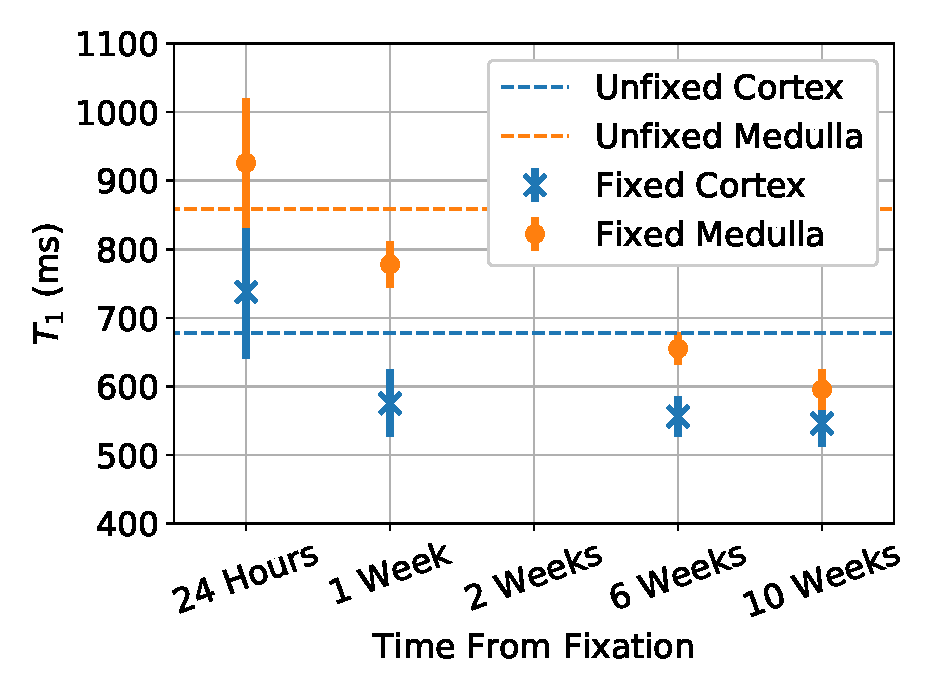
\includegraphics[width=1\textwidth]{Neph/T1_3T_crop.eps}
			\caption{}
			\label{fig:ex_fixation_t1_3t_lts}
		\end{subfigure}
		\hfill
		\begin{subfigure}[c]{0.47\textwidth}
			\centering
			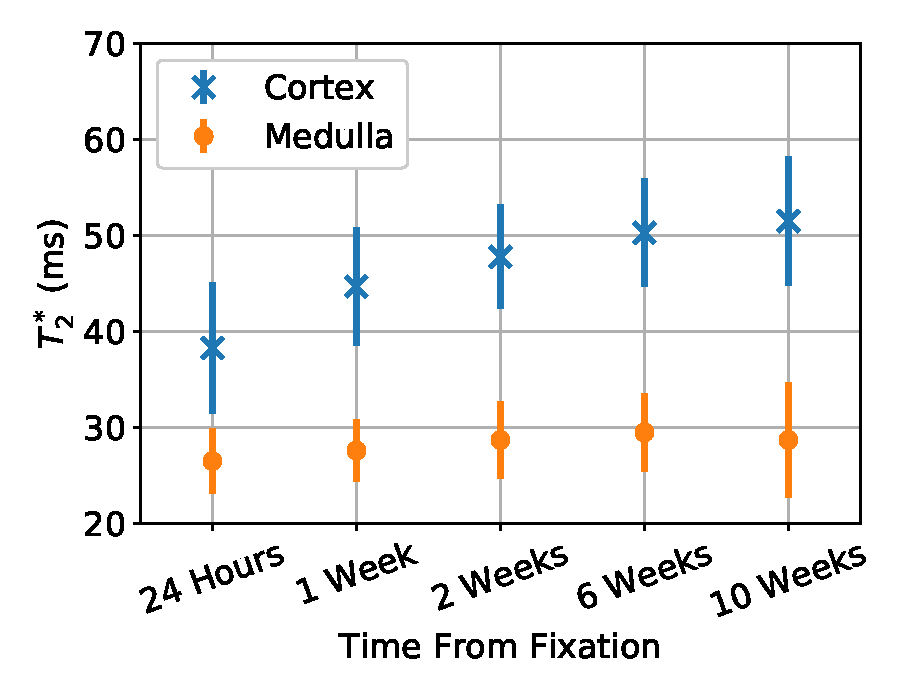
\includegraphics[width=1\textwidth]{Neph/T2star_3T_crop.eps}
			\caption{}
			\label{fig:ex_fixation_t2star_3t_lts}
		\end{subfigure}
	\end{subfigure}
	\vskip\baselineskip
	\begin{subfigure}[c]{0.9\textwidth}
		\centering
		\begin{subfigure}[c]{0.47\textwidth}
			\centering
			\includegraphics[width=1\textwidth]{Neph/T1_7T_crop.eps}
			\caption{}
			\label{fig:ex_fixation_t1_7t_lts}
		\end{subfigure}
		\hfill
		\begin{subfigure}[c]{0.47\textwidth}
			\centering
			\includegraphics[width=1\textwidth]{Neph/T2star_7T_crop.eps}
			\caption{}
			\label{fig:ex_fixation_t2star_7t_lts}
		\end{subfigure}
	\end{subfigure}
	\caption{(\subref{fig:ex_fixation_t1_3t_lts}) Variation in $T_1$ as a function of time after fixation measured at 3T (\subref{fig:ex_fixation_t2star_3t_lts}) Variation in $T_2^*$ as a function of time after fixation measured at 3T (\subref{fig:ex_fixation_t1_7t_lts}) Variation in $T_1$ as a function of time after fixation measured at 7T (\subref{fig:ex_fixation_t2star_7t_lts})  Variation in $T_2^*$ as a function of time after fixation measured at 7T.}
	\label{fig:ex_fixation_lts}
\end{figure}

\begin{figure}[H]
	\centering
	\begin{subfigure}[c]{0.47\textwidth}
		\centering
		\includegraphics[width=1\textwidth]{Neph/T1_map_STS.eps}
		\caption{}
		\label{fig:ex_fixation_t1map_3t_sts}
	\end{subfigure}
	\hfill
	\begin{subfigure}[c]{0.47\textwidth}
		\centering
		\includegraphics[width=1\textwidth]{Neph/T2star_map_STS.eps}
		\caption{}
		\label{fig:ex_fixation_t2starmap_3t_sts}
	\end{subfigure}
	\caption{(\subref{fig:ex_fixation_t1map_3t_sts}) An example of the $T_1$ map collected from the short time scale kidney (\subref{fig:ex_fixation_t2starmap_3t_sts}) An example of the $T_2^*$ map collected from the short time scale kidney.}
	\label{fig:ex_maps_sts}
\end{figure}

\begin{figure}[H]
	\centering
	\begin{subfigure}[c]{0.47\textwidth}
		\centering
		%		\missingfigure{T1 vs Times (STS)}
		\includegraphics[width=1\textwidth]{Neph/STS_T1_line.eps}
		\caption{}
		\label{fig:ex_fixation_t1_3t_sts}
	\end{subfigure}
	\hfill
	\begin{subfigure}[c]{0.47\textwidth}
		\centering
		%		\missingfigure{T2* vs Times (STS)}
		\includegraphics[width=1\textwidth]{Neph/STS_T2star_line.eps}
		\caption{}
		\label{fig:ex_fixation_t2star_3t_sts}
	\end{subfigure}
	\caption{(\subref{fig:ex_fixation_t1_3t_sts}) Variation in $T_1$ as a function of time after fixation measured at 3T (\subref{fig:ex_fixation_t2star_3t_sts}) Variation in $T_2^*$ as a function of time after fixation measured at 3T.}
	\label{fig:ex_fixation_sts}
\end{figure}

\begin{figure}[H]
	\centering
	\begin{subfigure}[c]{0.47\textwidth}
		\centering
		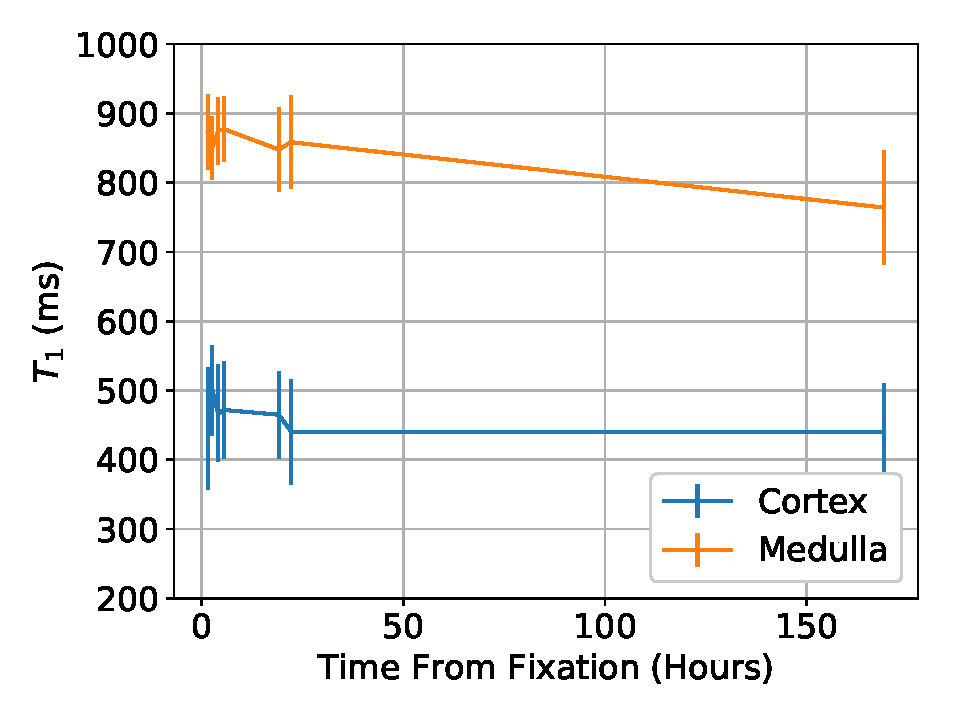
\includegraphics[width=1\textwidth]{Neph/MTS_T1_line.eps}
		\caption{}
		\label{fig:ex_fixation_t1_3t_mts}
	\end{subfigure}
	\hfill
	\begin{subfigure}[c]{0.47\textwidth}
		\centering
		\includegraphics[width=1\textwidth]{Neph/MTS_T2star_line.eps}
		\caption{}
		\label{fig:ex_fixation_t2star_3t_mts}
	\end{subfigure}
	\caption{(\subref{fig:ex_fixation_t1_3t_mts}) Variation in $T_1$ as a function of time after fixation measured at 3T (\subref{fig:ex_fixation_t2star_3t_mts}) Variation in $T_2^*$ as a function of time after fixation measured at 3T.}
	\label{fig:ex_fixation_mts}
\end{figure}
\section{Layer Based Analysis of Renal Data}
\label{sec:ex_layers}
% Motivation
% Methods
% Results
\begin{figure}[H]
	\centering
	\begin{subfigure}[c]{0.47\textwidth}
		\centering
		\includegraphics[height=1\textwidth]{Other/Layers/mri_to_roi_to_surf_Artboard_5.eps}
		\caption{}
		\label{fig:ex_layers_brain}
	\end{subfigure}
	\hfill
	\begin{subfigure}[c]{0.47\textwidth}
		\centering
		\includegraphics[height=1\textwidth]{Other/Layers/kidney_levelsets-02.eps}
		\caption{}
		\label{fig:ex_layers_kidney}
	\end{subfigure}
	\caption{(\subref{fig:ex_layers_brain}) A depth mask of the brain. Lighter areas are deeper inside the brain. (\subref{fig:ex_layers_kidney}) A depth mask applied to a quantitative $T_1$ map.}
	\label{fig:ex_layers_example}
\end{figure}

\section{Correlating MRI Measures with Histopathology in Aged Kidneys}
% Method
% Results

\begin{figure}[H]
	\centering
	\begin{subfigure}[c]{0.47\textwidth}
		\centering
		\includegraphics[width=1\textwidth]{Neph/aged_kidneys/Young_T1.eps}
		\caption{}
		\label{fig:ex_aged_t1_map}
	\end{subfigure}
	\hfill
	\begin{subfigure}[c]{0.47\textwidth}
		\centering
		\includegraphics[width=1\textwidth]{Neph/aged_kidneys/Old_T1.eps}
		\caption{}
		\label{fig:ex_aged_t2star_map}
	\end{subfigure}
	\caption{(\subref{fig:ex_aged_t1_map}) $T_1$ map of a 0.5 year old pig kidney. (\subref{fig:ex_aged_t2star_map}) $T_1$ map of a 2.5 year old pg kidney.}
	\label{fig:ex_aged_map}
\end{figure}

\begin{figure}[H]
	\centering
	\begin{subfigure}[c]{0.47\textwidth}
		\centering
		\includegraphics[width=1\textwidth]{Neph/aged_kidneys/T1_bar.eps}
		\caption{}
		\label{fig:ex_aged_t1_bar}
	\end{subfigure}
	\hfill
	\begin{subfigure}[c]{0.47\textwidth}
		\centering
		\includegraphics[width=1\textwidth]{Neph/aged_kidneys/T2star_bar.eps}
		\caption{}
		\label{fig:ex_aged_t2star_bar}
	\end{subfigure}
	\caption{(\subref{fig:ex_aged_t1_bar}) The $T_1$ of the renal cortex and medulla of the two samples. (\subref{fig:ex_aged_t2star_bar}) The $T_2^*$ of the renal cortex and medulla of the two samples.}
	\label{fig:ex_aged_bar}
\end{figure}

\begin{figure}[H]
	\centering
	\begin{subfigure}[c]{0.9\textwidth}
		\centering
		\begin{subfigure}[c]{0.47\textwidth}
			\centering
			\includegraphics[width=1\textwidth]{Neph/aged_kidneys/Figure_5_V3_Young_H_and_E.png}
			\caption{}
			\label{fig:ex_young_h_and_e}
		\end{subfigure}
		\hfill
		\begin{subfigure}[c]{0.47\textwidth}
			\centering
			\includegraphics[width=1\textwidth]{Neph/aged_kidneys/Figure_5_V3_Old_H_and_E.png}
			\caption{}
			\label{fig:ex_old_h_and_e}
		\end{subfigure}
	\end{subfigure}
	\vskip\baselineskip
	\begin{subfigure}[c]{0.9\textwidth}
		\centering
		\begin{subfigure}[c]{0.47\textwidth}
			\centering
			\includegraphics[width=1\textwidth]{Neph/aged_kidneys/Figure_5_V3_Young_Trichrome.png}
			\caption{}
			\label{fig:ex_young_trichrome}			
		\end{subfigure}
		\hfill
		\begin{subfigure}[c]{0.47\textwidth}
			\centering
			\includegraphics[width=1\textwidth]{Neph/aged_kidneys/Figure_5_V3_Old_Trichrome.png}
			\caption{}
			\label{fig:ex_old_trichrome}
		\end{subfigure}
	\end{subfigure}
	\caption{(\subref{fig:ex_young_h_and_e}) A sample of renal cortex from a 0.5 year old pig stained with \ac{H and E}. (\subref{fig:ex_old_h_and_e}) A sample of renal cortex from a 2.5 year old pig stained with \ac{H and E}. (\subref{fig:ex_young_trichrome}) A sample of renal cortex from a 0.5 year old pig stained with Masson's trichrome. (\subref{fig:ex_old_trichrome}) A sample of renal cortex from a 2.5 year old pig stained with Masson's trichrome.} 
	\label{fig:ex_aged_histo}
\end{figure}

\section{Conclusion}

\section{Acknowledgements}

We are grateful for access to the University of Nottingham's Augusta high performance computing service. We also thank Prof David Gardner of University of Nottingham Veterinary Science for his assistance with sample acquisition, histopathological processing of samples and general renal physiology expertise.

\newpage
\section{References}
\defbibheading{bibliography}[\refname]{}
\printbibliography